
\chapter{Jackknife Resampling}\label{ch-jack}

This paper is based on
Ref. \cite{wiki-jack}.

Before reading this chapter,
we recommend that you
read the section entitled
``Demystifying
Population and Sample
Variances", in
Chapter [\nameref{ch0-conventions}].

Jackknife Resampling (JR)
is a way of
generating from an
original list
of $n$ samples,
a new list of $n$ synthetic
(i.e., man made, not
occurring physically
in Nature) samples
obtained by deleting
one of the
samples from the original list
and
averaging over the rest.


Let $\Sigma=\{0,1,2, \ldots, n-1\}$.
Let us consider the list of samples

\beq
\vec{x}=(x^\s)_{\s\in\Sigma}
\;,
\eeq
where the $x^\s$ are assumed to be i.i.d. with


\beq
E[\rvx^\s]=\mu
\eeq
and

\beq
\av{\rvx^\s, \rvx^{\s'}}=V_1\delta(\s, \s')
\;.
\eeq
If we define $\mu$ and $V_1$
 estimators by

\begin{subequations}
\label{eq-jr-xs-estimators}
\beq
\hat{\mu}=\frac{1}{n}\sum_\s x^\s
\eeq

\beq
\hat{V}_1=
\frac{1}{n-1}\sum_\s (x^\s-\hat{\mu})^2
\;,
\eeq
\end{subequations}
then one can show that:

\beq
E[\ul{\hat{\mu}}]=\mu\;,\;\;E[\hat{\rvV}_1]=V_1
\eeq
so both of these estimators are unbiased.

Now define lists
of samples with one
of the items in $\vec{x}$ deleted:

\beq
\vec{x}_\xi=(x^\s)_{\s\in\Sigma-\{\xi\}}
\;.
\label{eq-def-vec-x-xi}
\eeq

Suppose we are given functions
of $\vec{x}$ and $\vec{x}_\xi$

\beq
A=A^n(\vec{x})
\;,
\eeq

\beq
A_\xi=A^{n-1}(\vec{x}_\xi)
\;.
\label{eq-def-a-xi}
\eeq
Then define a list $\vec{A}$ by
\beq
\vec{A}=(A_\xi)_{\xi\in \Sigma}
\;.
\eeq
One can also define a list
$\vec{B}$ by:

\beq
\vec{B}=
(B_\xi)_{\xi\in \Sigma}
\eeq
where

\beqa
B_\xi&=&
nA-(n-1)A_\xi\\
&=&
A_\xi
-n[A_\xi-A]
\;.
\label{eq-def-b-xi}
\eeqa
Later on,
we will see why
the list $\vec{B}$
just defined is of
interest.

\begin{figure}[h!]
$$
\xymatrix{
&\vec{\rvx}
\ar[lddd]
\ar[d]\ar[dr]\ar[drr]
\\
&\vec{\rvx}_0\ar[d]
&\vec{\rvx}_1\ar[d]
&\vec{\rvx}_2\ar[d]
\\
&\rvA_0\ar[d]
&\rvA_1\ar[d]
&\rvA_2\ar[d]
\\
\rvA\ar[r]
\ar@/_1pc/[rr]
\ar@/_1pc/[rrr]
&\rvB_0
&\rvB_1
&\rvB_2
}
$$
\caption{Bnet for jackknife resampling (JR).}
\label{fig-jack-bnet}
\end{figure}

Fig.\ref{fig-jack-bnet}
is a bnet
that encapsulates JR.
The TPMs, printed in blue,
for that bnet,
are as follows:

\beq\color{blue}
P(\vec{x}_\xi|\vec{x})=
\indi(\;\;\;
\vec{x}_\xi= \text{ defined by Eq.(\ref{eq-def-vec-x-xi})}
\;\;\;)
\eeq

\beq\color{blue}
P(A_\xi|\vec{x}_\xi)=
\indi(\;\;\;
A_\xi= \text{ defined by Eq.(\ref{eq-def-a-xi})}
\;\;\;)
\eeq

\beq\color{blue}
P(B_\xi|\vec{A}_\xi, A)=
\indi(\;\;\;
B_\xi= \text{ defined by Eq.(\ref{eq-def-b-xi})}
\;\;\;)
\eeq



\section{Case
$A=A^n(\vec{x})=\frac{1}{n}
\sum_\sigma x^\sigma$}

Suppose

\beq
A=
\underbrace{\frac{1}{n}\sum_\s x^\s}_
{ E_\s[x^\s]}
\eeq
and

\beq
A_\xi=
\underbrace{\frac{1}{n-1}
\sum_{\s\in \Sigma-\{\xi\}}
 x^\s}_
{E_{\s|\xi}[x^\s]\text{ where } P(\s|\xi)=\frac{\indi(\s\neq\xi)}{n-1}}
\;.
\eeq
Then

\beq
\frac{1}{n}
\sum_\xi
A_\xi=E_\xi E_{\s|\xi}[x^\s]=E_\s[x^\s]=A
\eeq

\begin{claim}
\beq
E[\rvA_\xi]=\mu
\eeq

\beq
\av{\rvA_\xi, \rvA_{\xi'}}=
V_1
\left[
\frac{n-2-\delta(\xi, \xi')}{n-1}
\right]
\eeq
\end{claim}
\proof
\beqa
E[\rvA_\xi]=\frac{1}{n-1}\sum_\s \indi(\xi\neq\s)E[\rvx^\s]=\mu
\eeqa

\beqa
\av{\rvA_\xi, \rvA_{\xi'}}&=&
\frac{1}{n-1}
\sum_\s\sum_{\s'}
[1-\delta(\s, \xi)]
[1-\delta(\s', \xi')]\av{x^\s, x^{\s'}}
\\
&=&
\frac{V_1}{n-1}
\sum_\s\sum_{\s'}
[1-\delta^\s_\xi-\delta^{\s'}_{\xi'}
+
\delta^\s_\xi\delta^{\s'}_{\xi'}]\delta^\s_{\s'}
\\
&=&
\frac{V_1}{n-1}
[n-2+\delta^\xi_{\xi'}]
\eeqa
\qed

\begin{figure}[h!]
\centering
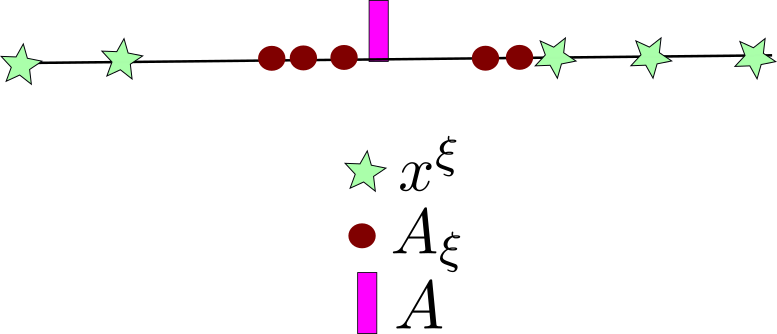
\includegraphics[width=2in]
{jack/jack-dots.png}
\caption{For each
point $x^\xi$,
there  is a corresponding point
$A_\xi$
which is $n-1$ times closer to the average $A$
than $x^\xi$ is.}
\label{fig-jack-dots}
\end{figure}

\begin{claim}
\beq
A_\xi-A=
\frac{A-x^\xi}{n-1}
\label{eq-prox-to-A}
\eeq
Hence, the distance of a point
$x^\xi$ to the mean value  $A$
is $n-1$ times as large
as the distance of $A_\xi$ to $A$.
(see Fig.\ref{fig-jack-dots})
\end{claim}
\proof
\beqa
A_\xi-A
&=&
\frac{1}{n-1}
\left(\sum_\s x^\s - x^\xi\right)
-
\frac{1}{n}\sum_\s x^\s
\\
&=&
x^\xi\left(\frac{-1}{n-1}\right)
+
\sum_\s x^\s
\underbrace{\left(
\frac{1}{n-1}-
\frac{1}{n}\right)}_
{\frac{1}{n(n-1)}}
\\
&=&
\frac{A-x^\xi}{n-1}
\eeqa
\qed

Note that
\beq
(n-1)\sum_\xi (A_\xi-E_\xi[A_\xi])^2
=
\hat{V}_1
\eeq
by Eq.(\ref{eq-prox-to-A}).
Hence, we can estimate
$V_1$ from $\vec{A}$
instead of $\vec{x}$.

Note that
\beqa
B_\xi&=&nA-(n-1)A_\xi
\\
&=&
\sum_\s x^\s-\sum_{\s\neq \xi}x^\s =x^\xi
\eeqa
Since $B_\xi=x^\xi$,
they have identical statistics.
In particular, one can use for
$B_\xi$ the same $\mu$ and $V_1$ estimators that we
defined in Eqs.(\ref{eq-jr-xs-estimators}) for $x^\s$.
